% Section 3 - Message topics
% Roberto Masocco <roberto.masocco@uniroma2.it>
% April 23, 2025

% ### Message topics ###
\section{Message topics}
\graphicspath{{figs/section3/}}

% --- ROS 2 messages ---
\begin{frame}{ROS 2 messages}
	A message is a \textbg{single data packet} sent over a \textbg{topic}, from \textbg{publisher nodes} to \textbg{subscriber nodes}, with a specific \textbg{QoS policy}.
	\begin{figure}
		\centering
		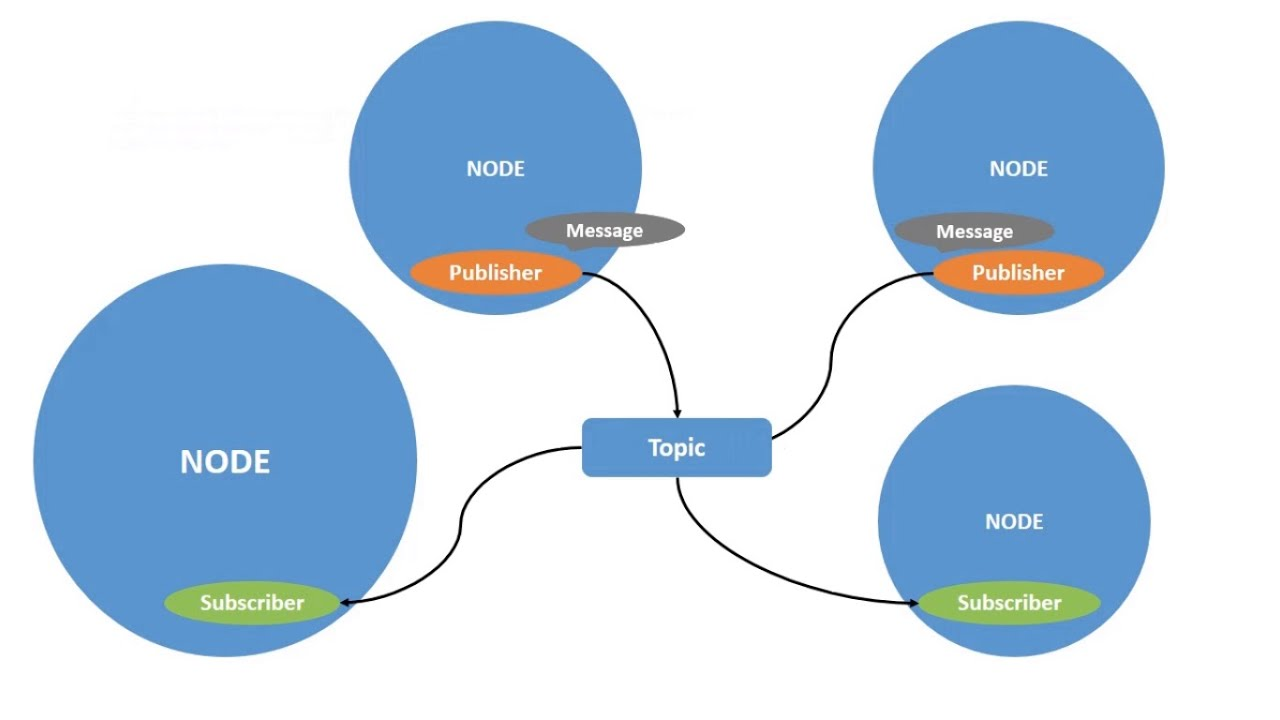
\includegraphics[scale=.16]{ros2Msg.jpg}
		\caption{Example of a topic with multiple publisher and subscriber nodes.}
		\label{fig:msg}
	\end{figure}
  Figure \ref{fig:msg} is also an example of a simple \textbg{node graph}, a pivotal concept in a distributed context.
\end{frame}

% --- Interface files - Messages ---
\begin{frame}[fragile]{Interface files}{Messages}
	Interface files format is \textbg{derived from the DDS standard}, with data types resolved to machine types according to the platform being used\footnote{\href{https://docs.ros.org/en/jazzy/Concepts/About-ROS-Interfaces.html}{\color{blue}\underline{About ROS 2 interfaces}} (ROS 2 Jazzy docs)}.\\
	Message file names end with \textbg{\texttt{.msg}}.\\
	Things start very simply...

	\begin{columns}
		\column{.9\textwidth}
		% Listing: std_msgs/msg/Int64 message definition
		\begin{lstlisting}[language=ros2msg, caption=Definition of the \texttt{std\_msgs/msg/Int64} message.]
int64 data\end{lstlisting}

		% Listing: std_msgs/msg/String message definition
		\begin{lstlisting}[language=ros2msg, caption=Definition of the \texttt{std\_msgs/msg/String} message.]
string data\end{lstlisting}
	\end{columns}

\end{frame}
\begin{frame}[fragile]{Interface files}{Messages}
	... then escalate quickly!

	\begin{columns}
		\column{.9\textwidth}
		% Listing: sensor_msgs/msg/Image
		\begin{lstlisting}[language=ros2msg, caption=Definition of the \texttt{sensor\_msgs/msg/Image} composite message.]
std_msgs/Header header
# ^ This includes another message type as a sub-structure

uint32 height
uint32 width

string encoding

uint8 is_bigendian
uint32 step
uint8[] data # This specifies a variable-length uint8 array\end{lstlisting}
	\end{columns}

\end{frame}
\begin{frame}[fragile]{Interface files}{Messages}
	Special values (\emph{i.e.}, \textbg{constants}) or \textbg{default values} may be specified.

	\begin{columns}
		\column{.9\textwidth}
		% Listing: message with constant
		\begin{lstlisting}[language=ros2msg, caption=Definition of an example message with a constant and a default value.]
int64 MYNUM=1 # Must be of compatible type

int64 number
int64 number_with_default 2\end{lstlisting}
	\end{columns}

	They are not bound to any field and will appear as \textbg{special selectable values} in the generated C++/Python libraries code.\\
	ROS 2 adds its own \textbg{guidelines}\footnote{\href{https://github.com/IntelligentSystemsLabUTV/ros2-examples/blob/jazzy/interfaces.md}{\color{blue}\underline{ros2-examples/interfaces.md}}}, and installed interfaces can be inspected with\\
  \medskip
	\texttt{ros2 interface show}
\end{frame}

% --- Message topics - Quality of Service ---
\begin{frame}{Message topics}{Quality of Service}
	A \textbg{QoS policy} for publishers/subscribers is a data structure with the following attributes:
	\begin{itemize}
		\item \textbg{History} (\emph{keep last N} or \emph{all})
		\item \textbg{Depth} (queue size \emph{N})
		\item \textbg{Reliability} (\emph{best-effort} or \emph{reliable}, default: reliable)
		\item \textbg{Durability} (publishers resend all messages to "late-joiners")
		\item Deadline
		\item \textbg{Lifespan} (message expiration date)
		\item Liveliness
		\item Lease duration
	\end{itemize}
	Default \textbg{profiles} are available (e.g. \textbg{Sensor data}, \textbg{Service}...), see the \href{https://docs.ros.org/en/jazzy/Concepts/About-Quality-of-Service-Settings.html}{\color{blue}\underline{docs}}.
\end{frame}
\begin{frame}{Message topics}{Inspection tools}
  The command line tool \texttt{ros2 topic} can be used to \textbg{inspect topics} and related entities.\\
  It has a lot of \textbg{verbs}, the most important ones are:
  \begin{itemize}
    \item \texttt{list} (list all topics)
    \item \texttt{echo} (print messages to the console)
    \item \texttt{pub} (publish messages from the console)
    \item \texttt{hz} (print publishing rate and statistics)
    \item \texttt{info} (print information about a topic)
    \item \texttt{type} (print the message type)
  \end{itemize}
  each with many useful options.\\
  \textbg{Nodes} can be inspected with the \texttt{ros2 node} command, and its many verbs.
\end{frame}

% --- Example - Topic pub/sub ---
\begin{frame}{Example}{Topic pub/sub}
  \begin{block}{}
    \centering
	  Now go have a look at the first two example packages:\\
    \href{https://github.com/IntelligentSystemsLabUTV/ros2-examples/tree/jazzy/src/cpp/topic_pubsub_cpp}{\color{blue}\underline{ros2-examples/src/cpp/topic\_pubsub\_cpp}}\\
    \smallskip
    \href{https://github.com/IntelligentSystemsLabUTV/ros2-examples/tree/jazzy/src/python/topic_pubsub_py}{\color{blue}\underline{ros2-examples/src/python/topic\_pubsub\_py}}
  \end{block}
\end{frame}

% --- Exercises ---
\begin{frame}{Exercises}
  \begin{itemize}
    \item Install ROS 2 on a platform of your choice.
    \item Run the \href{https://docs.ros.org/en/jazzy/Installation/Ubuntu-Install-Debs.html\#try-some-examples}{\color{blue}\underline{demo nodes}}.
    \item Inspect the demo topics.
    \item Interact with the demo nodes from the command line.
    \item Clone \href{https://github.com/IntelligentSystemsLabUTV/ros2-examples}{\color{blue}\underline{\texttt{ros2-examples}}} as suggested and rebuild the first example packages.
    \item Listen to the \texttt{/rosout} topic from the command line while other nodes run.
  \end{itemize}
\end{frame}
